\documentclass[12pt]{article}

% https://www.rit.edu/research/srs/sites/rit.edu.research.srs/files/mission_agencies_workshop_rfp_2019.pdf

\usepackage{cite}
\usepackage{listings}
\usepackage{times}
\usepackage{color}
\usepackage{url}
\usepackage{multirow}
\usepackage{enumitem} % Use for enumerating A, B, C etc...
\urlstyle{same} % Used for formatting formatting url footnotes
\usepackage{fancyhdr} % Header
%\usepackage[table]{xcolor}% http://ctan.org/pkg/xcolor
\usepackage[table,xcdraw]{xcolor}
\usepackage{soul} % highlighting
%\usepackage{pgfgantt} % Project timeline
\usepackage[titletoc,toc,title]{appendix} % Need for appendix, page numbering
\usepackage{tikz}
\usetikzlibrary{calc,arrows.meta,fit,positioning}
%\usepackage{amssymb,graphicx} % Events and milestones
\usepackage{amsmath}
\usepackage{mathtools}
\usepackage{bbm}
\usepackage{amssymb}
\usepackage{booktabs} % used for \toprule in tables
\usepackage{wrapfig,booktabs} % Wrap text around table
\usepackage{booktabs} % used for \toprule in tables
\usepackage[table,xcdraw]{xcolor}
\DeclarePairedDelimiter\ceil{\lceil}{\rceil}
\DeclarePairedDelimiter\floor{\lfloor}{\rfloor}      
\usepackage[final]{pdfpages}
\usepackage{tocloft} % Table of contents spacing
\usepackage{xcolor,colortbl} %%% Color Table Header

\usepackage{makecell}

%\usepackage{subcaption} % Side by side images
%\usepackage{pgfplots} % Bar chart. Graph

\usepackage{xspace} % Needed for et al.
%\newcommand{\etal}{{et al.\@\xspace}} 
\newcommand{\etal}{\emph{et~al.}\xspace} 

\usepackage[bottom=1in, left=1in, right=1in, top=1in]{geometry} 

\usepackage[english]{babel}
\usepackage[utf8x]{inputenc}
\usepackage{graphicx}
\usepackage{wrapfig}
%\usepackage{lipsum}
%\usepackage{pgfgantt}

%\usepackage{minted} % Side by side code


% DK 10/30 Look at removing these
%\usepackage[textwidth = 155mm]{geometry}
%\usepackage{tabularx}


\newcommand{\todo}[1]{\textcolor{cyan}{\textbf{[#1]}}}
\newcommand{\dan}[1]{\textcolor{blue}{{\it [Dan says: #1]}}}
\newcommand{\qi}[1]{\textcolor{red}{{\it [Qi says: #1]}}}
\newcommand{\sakshi}[1]{\textcolor{green}{{\it [Sakshi says: #1]}}}


%%% Start column formatting
% Note: In overleaf sometimes columns fail to render. Check on PDF Output
\newcolumntype{L}[1]{>{\raggedright\arraybackslash}m{#1}} % raggedright= align left
\definecolor{Gray}{gray}{0.80} % the lower the #, the darker it gets
%%% End Table formatting

%%%% Start toggling showing/hiding some information
\newif\ifShowAll
\ShowAlltrue % Display All Info
%\ShowAllfalse % Hide Some Info





%\newcommand{\Title}{Uncertainty Reduction in Self-Adaptive Systems to Increase System Effectiveness, Efficiency and Resiliency} 
%\newcommand{\shortTitle}{Dynamic Bayesian Matrix Factorization for Uncertainty Reduction} 

% Dynamic Bayesian Matrix Factorization and Dynamic Assurance Cases for Uncertainty Reduction in Self-Adaptive Systems


%\newcommand{\Title}{Dynamic Bayesian Matrix Factorization and Dynamic Assurance Cases for Uncertainty Reduction in Self-Adaptive Systems} 
\newcommand{\Title}{Dynamic Bayesian Matrix Factorization and Dynamic Assurance Cases for Uncertainty Reduction in Self-Adaptive Systems}
\newcommand{\shortTitle}{Uncertainty Reduction in Self-Adaptive Systems} 


\newcommand{\CallNumber}{Mission Agencies Proposal Development Workshop 2019}
\newcommand{\CallName}{BBBB}

\usepackage{fancyhdr} % Header
\pagestyle{fancy}
\lhead{\emph{\shortTitle}}
\rhead{Krutz (RIT)}
%\lhead{\shortTitle}
%\rhead{}



\usepackage{lastpage}

\setlength\cftparskip{-.7pt} %% Table of contents spacing
%\setlength\cftbeforechapskip{0pt}

\begin{document}

\begin{titlepage}

\newcommand{\HRule}{\rule{\linewidth}{0.3mm}} % Defines a new command for the horizontal lines, change thickness here

%%%%%%% Start new Title format


%% DK: I am not sure if we should have this
%\noindent\large \CallName, \CallNumber\\[.20cm] % Call Name

\noindent\large \CallNumber\\[.20cm] % Call Name

\noindent \LARGE \textbf{\Title}\\[.10cm] % Title
%\noindent \LARGE \textbf{XXXXXDynamic Bayesian Matrix Factorization for~~~~~~~~~~~~~                   ~~~~          ~~~~~~~~~~~~    ~~~~~~~~~~~~~       ~~~~~    ~~~~XXUncertainty Reduction in Self-Adaptive SystemsXXXXX}\\[.10cm] % DK: Nasty, but this takes care of the word wrap problem




%\noindent \large  \underline{\textbf{Technical Proposal}}\\ [.15cm] 

\begin{tabular}{ L{15mm} L{120mm} }

%\normalsize \textbf{Technical Proposal:} & \normalsize  \CallName, \CallNumber  \\

%\noindent\large Technical Proposal: N00174-18-0001\\[.20cm]
%\noindent\large NEC Technical POC: \\[.20cm]
%\noindent\large Topic Number: \\[.20cm]




\normalsize \textbf{PI:} & \normalsize  Dr. Daniel Krutz \\
    & \vspace{-6mm} \normalsize Assistant Professor \\
    & \vspace{-12mm} \normalsize Department of Software Engineering \& Center of Cybersecurity
 \\
   & \vspace{-18mm} \normalsize Golisano College \\
   & \vspace{-24mm} \normalsize Email: dxkvse@rit.edu \\


%\normalsize \textbf{Co-PI:} & \normalsize  Dr. Qi Yu \\
%    & \vspace{-6mm} \normalsize Associate Professor \\
%    & \vspace{-12mm} \normalsize Information Sciences and Technologies Department
% \\
%   & \vspace{-18mm} \normalsize Golisano College \\
%   & \vspace{-24mm} \normalsize Email: qi.yu@rit.edu \\



\end{tabular}




 \end{titlepage}

\cfoot{\thepage}
\pagenumbering{alph} % Start roman numbering
\setcounter{tocdepth}{1} % Show sections

\cfoot{} % Leave blank

% https://texblog.org/2013/04/29/latex-table-of-contents-list-of-figurestables-and-some-customizations/


%\tableofcontents
%\addtocontents{toc}{~\hfill\textbf{Page}\par}
%\chapter{...}

%\renewcommand\contentsname{Table of Contents}



%\tableofcontents
%\vspace{-6mm}
%\listoffigures
%\vspace{-4mm}
%\listoftables
%\newpage

\setcounter{page}{1}
\pagenumbering{arabic} % Switch to normal numbers

%\cfoot{\thepage\ of \pageref{LastPage}}
\fancyfoot[C]{Page~\thepage~of~\pageref{lastpage}}


\section*{Overview}

Tactics are the decisions made by self-adaptive systems to react to internal or external events, while continuing meet its objectives. Tactics encounter \emph{uncertainty} in terms of the latency, availability or dependability of the tactic. This uncertainty inhibits the creation of accurate and trustworthy information used in the decision-making process of self-adaptive systems. This project will reduce uncertainty in self-adaptive systems in two new and innovative ways: (I) Through the creation of a dynamic Bayesian matrix factorization framework to predict tactic volatility, which will enable the system to make more accurate tactic predictions (II) Assure tactic functionality through dynamically generated unit tests.


%100 Word Overview. Provide 1) an overview of the activity and a statement about the objectives and methods to be employed, 2) a statement on the intellectual or scientific merit of the proposed activity to advance knowledge and solve problems, 3) a statement on the relevance of the proposed activity to the targeted mission agency or program(s), and potential benefits of project outcomes. Suggested length: one half page.


\vspace{-5mm}
\section{Heilmeyer’s Questions} % ?Change name of this


\vspace{-0mm}\paragraph{What are you trying to do?}
%Self-adaptive systems rely upon accurate information 


The objective of this research is to investigate and demonstrate methods of reducing uncertainty in self-adaptive systems to provide more accurate information to the self-adaptive process. This will be accomplished through the use of a dynamic Bayesian matrix factorization model to predict tactic volatility and using dynamic assurance cases to ensure tactic functionality. This innovative work will \ul{increase the system's resiliency, efficiency, and ability to complete mission-critical operations}.

\vspace{-4mm}
%\subsection*{What is the current practice?}
\vspace{-0mm}\paragraph{What is the current practice?} 

% How are self-adaptive systems limited
Current decision-making processes are limited since they merely consider all tactics to have static attributes, regardless of internal or external variability encountered by the system. This can be problematic since in real-world scenarios, tactics may have highly volatile, evolving attributes. Not accounting for tactic volatility creates uncertainty in the decision-making process. State of the art self-adaptive processes are restricted in that they do not allow self-adaptive systems to learn from their previous tactic experiences. For example, a system may assume that it always takes 2 seconds to conduct a specific action, when in reality it has been observed to consistently take 4 seconds. If unable to learn, this means that the system will continually make decisions based upon inaccurate information. Current adaptation processes are unable to adapt and learn from tactic experiences and will continue to assume that the tactic continues to take the pre-defined, inaccurate amount of time to execute. Additional forms of tactic volatility include dependability and availability. We will next present examples of each form of tactic volatility, and how they can be detrimental to the self-adaptive process.


%Assurance cases are becoming more widely recognized as a necessity to ensuring system functionality and resiliency~\cite{weyns2017perpetual, schmerl2017challenges, de2017software}. 

% Assurance cases
An \emph{assurance} for a self-adaptive system may be defined as ``providing evidence for requirements compliance''~\cite{weyns2017perpetual}. Assurance cases are quickly becoming a recognized necessity for ensuring the functionality and resiliency of a self-adaptive system~\cite{schmerl2017challenges, de2017software}. This is especially true in mission or safety critical devices. While some works are beginning to enable systems to autonomously generate and execute assurance cases~\cite{denney2017tool}, the majority are limited in that that they still require significant human involvement~\cite{weyns2017perpetual}.


\vspace{-5mm}\paragraph{What is new in your approach and why do you think this will be successful?}

%% TVA approach \emph{Tactic Volatility Aware} (TVA)
Dynamic Bayesian matrix factorization is a proven approach for providing robust recommendations~\cite{sun2012dynamic}. This prediction model assumes that there are a number of common factors, including both observable and latent. Self-adaptive systems frequently encounter both of these types of factors, and it must account for them as effectively as possible. Our work is innovative since there has not even been an attempt to incorporate machine learning into the self-adaptive control loop to enable the system to learning for observed variability. 

A key challenge for self-adaptive systems is how to automatically ensure that the adapted system will provide the expected functionality. To help reduce this uncertainty, we will utilize concolic analysis~\cite{Sen:2005:CCU:1081706.1081750} to automatically create unit tests for the system's functionality, and match the possible software inputs against the expected outputs. Concolic analysis will automatically identify variable groups that are needed to ensure that all possible paths of functionality are taken. By using the values from these groups, the system will be able to correlate the expected functionality from the requirements against the actual system functionality. Not only will this process remove the requirement for the humans in creating the test, but will importantly discover adaptation processes that would have otherwise been missed. No known efforts in assurance cases have attempted a dynamic assurance creation approach such as this.


%The proposed work in dynamic assurance cases utilizes concolic analysis, which has proven its ability \todo{cite} in a wide-range of previous research. Many of these works closely support the proposed effort. There is currently a lack of processes that dynamically generate assurance cases in self-adaptive systems. None of which utilize concolic analysis\todo{cite}.

%Self-adaptive systems are limited by their ability in assuring their functionality, and too frequently require 


%The current body of knowledge of assurance cases is limited by a lack of 

% latent and observed variables





% Proven approach for learning



%% Assurance cases




% Proof of concept works have demonstrated the success



\vspace{-5mm}\paragraph{What is the significance of your research if successful?} The project can positively impact large numbers of autonomous systems in terms of resiliency, efficiency and effectiveness. Self-adaptive systems will continue to become more ubiquitous, fulfilling a variety of new and different tasks. As these systems become more prevalent, the demand for better decision-making mechanisms in these systems will also grow. Our tactic volatility prediction process will easily integrate into existing adaptation control loops such as MAPE-K, making it adoptable by a large number of self-adaptive and intelligent systems. Our dynamic assurance cases will enable self-adaptive systems to better predict and understand adaptations that were performed incorrectly by the system. This will enable the system to (I) Avoid adaptation processes that have be identified as problematic (II) Perform possible actions to repair these issues.

%These results will be disseminated in publications and workshops at venues such as ICSE, FSE, AAAI and SEAMS.



\vspace{-5mm}\paragraph{What are the risks and how will you mitigate those risks? }Self-adaptive systems frequently operate in new environments, where existing data is limited or sparse. This lack of empirical data could limit the applicability in these scenarios. One method of addressing this concern is through the use of uncertainty reduction tactics~\cite{moreno2018uncertainty}. When very limited amounts of data are available, our approach will automatically revert to using predefined tactic values until an adequate amount of data has been collected.

%One concern is that systems should not merely focus on reducing uncertainty, but should also ensure that they are completing essential tasks/missions. Overly focusing on just reducing uncertainty/risk could potentially lead to systems that were overly conservative. Another challenge to our approach revolves around the $P$ component of our utility equation. Although we are able to factor in how many tactics are estimated to complete in a sequence, simply taking that percentage may not adequately represent real-world scenarios. For example, there may be certain tactics that simply don't work in specific environments. Therefore, it would be a waste of resources to estimate those tactic's utility when we already know it won't work. 


% The cost of using this prediction model could outweigh the possible benefits

% Might not have enough data in some situations


% Concolic analysis




\vspace{-5mm}\paragraph{What are the metrics for success for your research? }Our approach will be evaluated by comparing it against existing methodologies using several data sets including those from The Internet Traffic Archive'~\cite{InternetTrafficArchive_URL} and `SEAMS Exemplars'~\cite{SEAMS_Exemplars_URL}. We will use simulations in \emph{R}, and using tools such as SWIM~\cite{moreno2018swim} and RUBiS~\cite{Rubis_URL}. This will enable us to demonstrate the abilities of our proposed technique against leading existing processes. We will demonstrate the abilities of our dynamic assurance process through several proof of concept evaluations using custom-built prototypes and by also implementing this process into SWIM and RUBiS. We will seed random adaptation failures and evaluate the ability of our process to detect these failures.


%To evaluate our dynamic assurance process, we will








%i. What are you trying to do?
%ii. What is the current practice?
%iii. What is new in your approach and why do you think this will be successful?
%iv. What is the significance of your research if successful?
%v. What are the risks and how will you mitigate those risks?
%vi. What are the metrics for success for your research? 





\vspace{-5mm}
\section{Targeted Programs} There are innumerable sources of DOD funding for this research. Some of which include: 

\begin{itemize}[noitemsep]

\item ARL - W911NF-170-S-0003 - ``Intelligent Systems For Improved Decision Making" TPOC: Cliff Wang


\item AFRL- AFOSR-2016-007 - ``Science of Information, Computation, Learning, and Fusion'' -  Richard (Doug) Riecken

%https://www.onr.navy.mil/-/media/Files/Funding-Announcements/BAA/2018/N00014-18-S-B001.ashx

\item AFRL - AFRL-RIK-2016-0005 - ``Resilient Autonomous Systems'' -  TPOC - Vincent Guza

\item ONR - N00014-18-S-B001 - ``Science of Autonomy'' - TPOC: Marc Steinberg 


\end{itemize}





%%%%%

%ARL BAA \# W911NF-170-S-0003 ``Autonomous Agents''' TPOC: 
% https://www.arl.army.mil/www/pages/8/W911NF-17-S-0003.pdf


% Check these (provide citations for all of these)

% https://www.grants.gov/web/grants/view-opportunity.html?oppId=295281
% https://www.grants.gov/web/grants/view-opportunity.html?oppId=297771
% https://www.grants.gov/web/grants/view-opportunity.html?oppId=305996



% Look at different BAAs that can be submitted to - Mention them by name/cite?
%


%This section should identify specific mission agencies, programs, and program officers or TPOCs with which the applicant will engage with as a result of the seed funding.



% Break this down by year
\vspace{-0mm} 
%\noindent \textbf{Total Requested Amount \emph{(3 years)}: }\$XX,XXX



%\vspace{2mm} \noindent \textbf{Requested Amount: }Travel Support is requested to meet with a TPOC, PO or attend a DOD Open Campus program. \dan{keep this section?}

%Yr 1 –\$54,571, Yr 2--\$49,571, Yr 3--\$49,847; Total: \$153,989 





%%%%%%%%%%%%%%%%%%%%%%%%%%%%%%%%

\label{lastpage}
\cleardoublepage


\appendix

\setcounter{page}{1}

%\addcontentsline{toc}{subsection}{Project Schedule}
\cfoot{\thepage}
\pagenumbering{roman}
%\section{Appendix}

%\input{sections/Appendix.tex}



%% I think the appendix goes before the bib. Otherwise, I could see people missing it
\newpage
\pagebreak
\addcontentsline{toc}{section}{References}
\bibliographystyle{plain}
\bibliography{refs}

\pagebreak


%\section{Attached CVs}
%\label{sec: attachedCVs}
%\vspace{-20mm}
\addcontentsline{toc}{section}{Attached CVs}
%   DK: Add these back in
%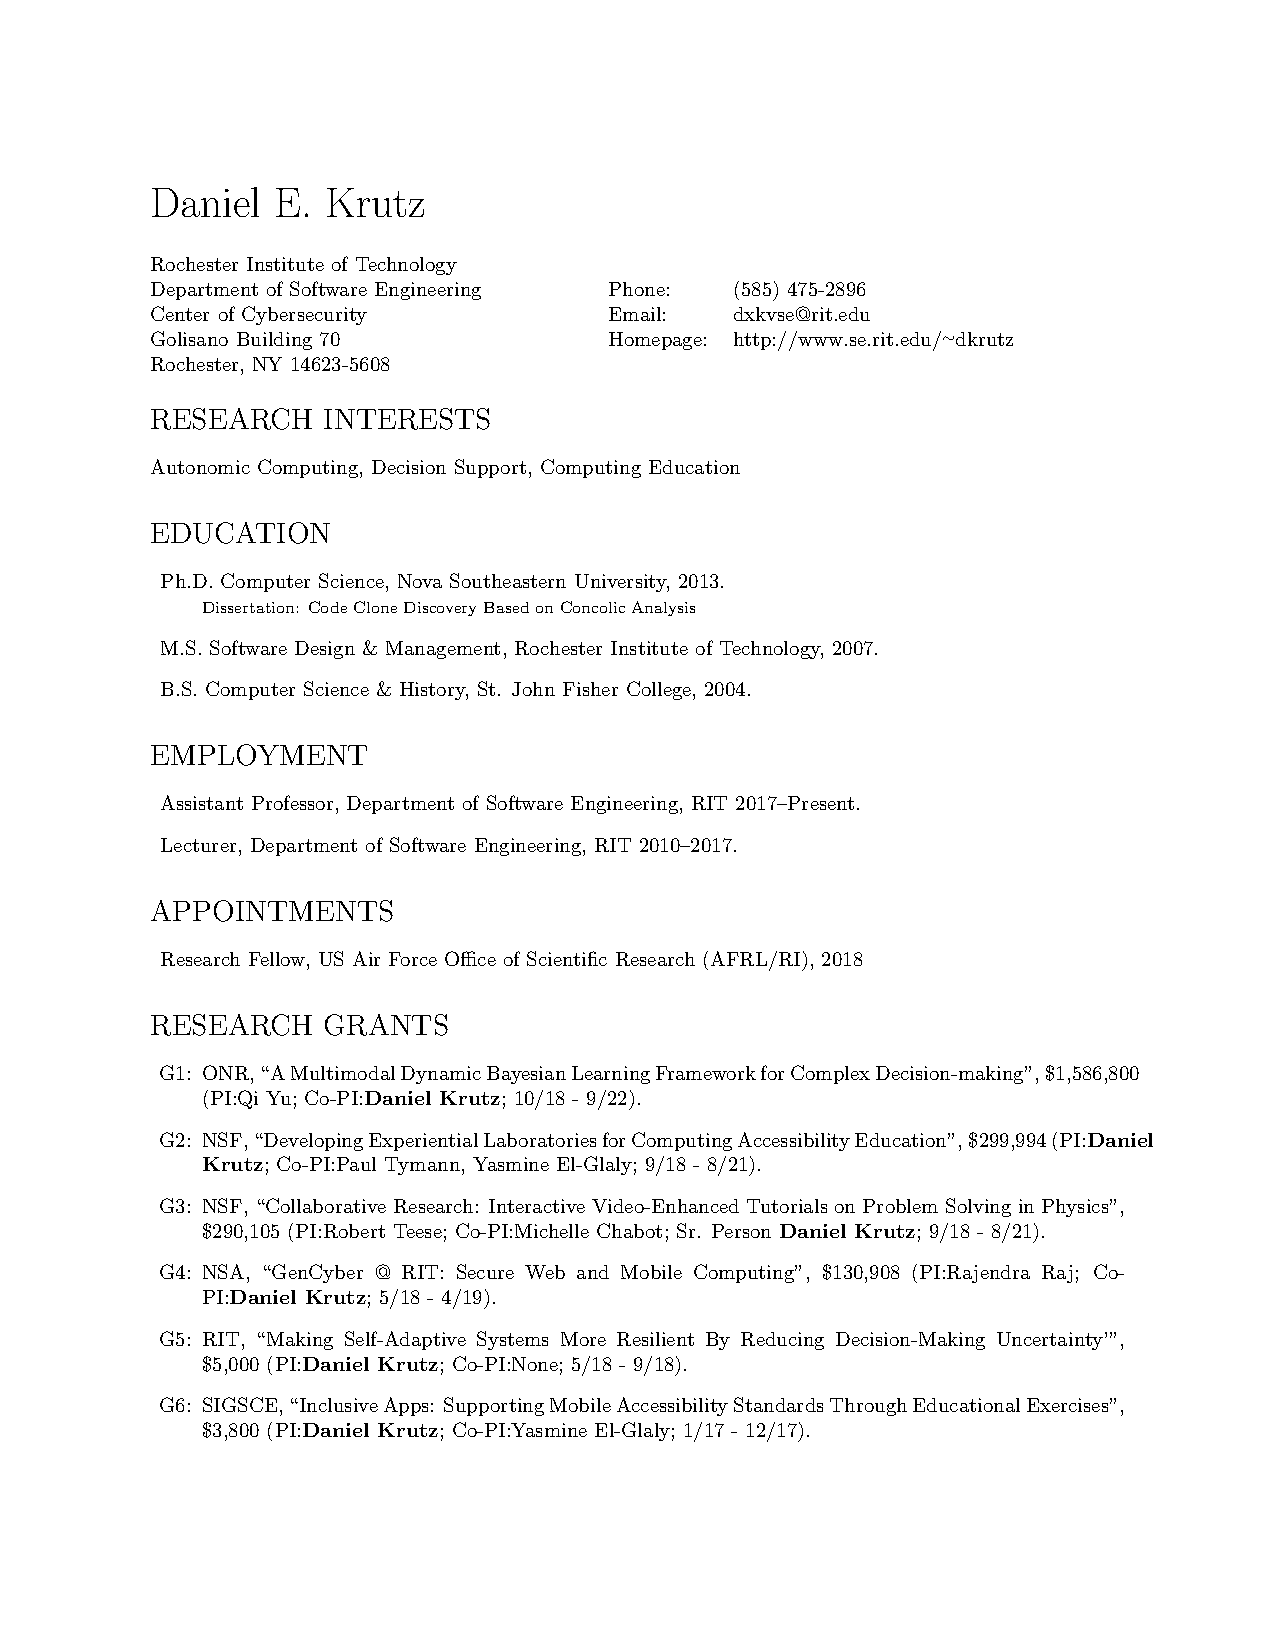
\includepdf[pages=-]{documents/cvs/Krutz_CVFull.pdf}
%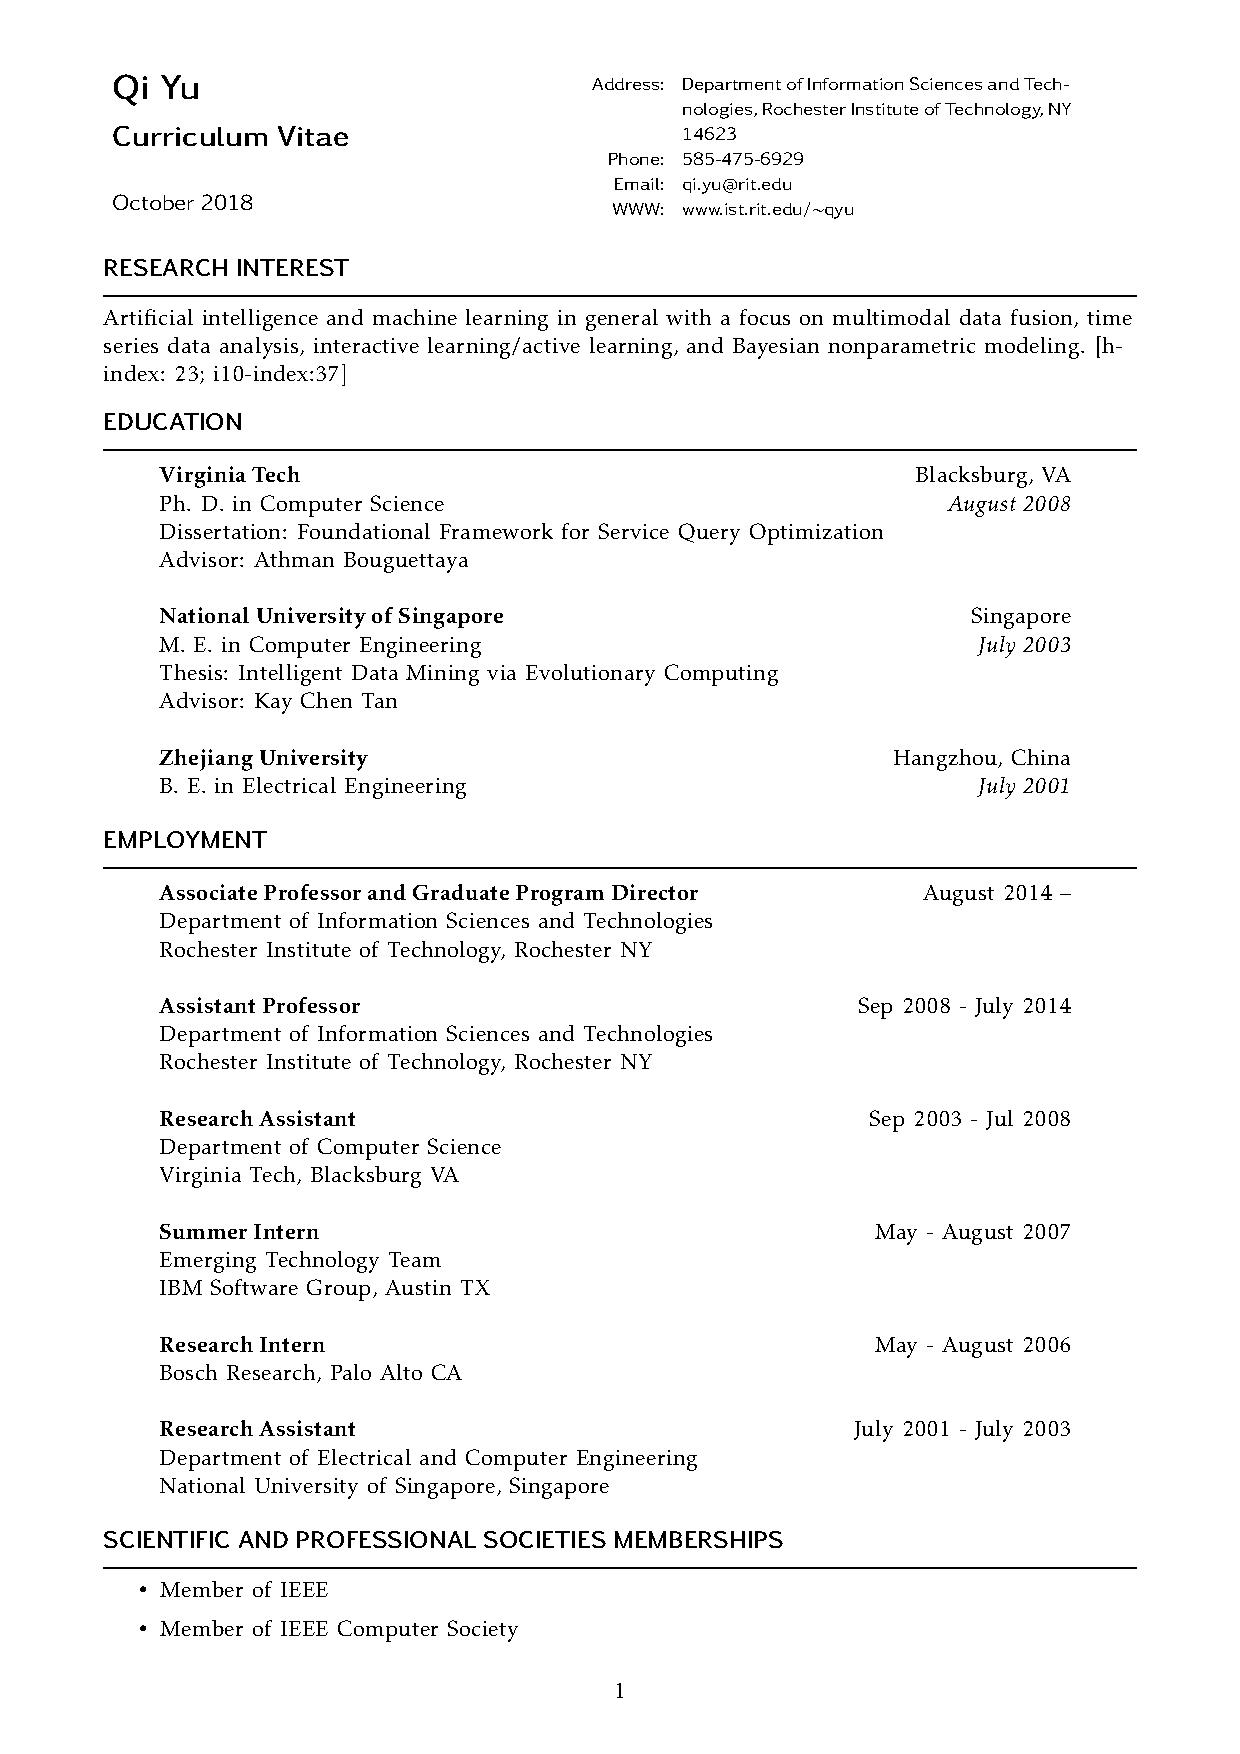
\includepdf[pages=-]{documents/cvs/Yu_CVFull.pdf}


\end{document}



% https://www.rit.edu/research/srs/sites/rit.edu.research.srs/files/mission_agencies_workshop_rfp_2019_0.pdf